\documentclass[a4paper]{article}

\usepackage[fontset=fandol]{ctex}
\usepackage{amsmath, amssymb}
\usepackage{graphicx}
\usepackage[margin=2.5cm]{geometry}
\usepackage[most]{tcolorbox}
\usepackage{etoolbox}
\usepackage{listings}
\usepackage{xcolor}
\usepackage{hyperref}
\usepackage{booktabs}
\usepackage{subcaption}
\usepackage{float}
\usepackage{tikz}
\IfFileExists{pgfplots.sty}{
    \usepackage{pgfplots}
    \pgfplotsset{compat=1.18}
}{}

\newtcolorbox{knowledgebox}[1]{
    enhanced, colback=blue!5!white, colframe=blue!75!black, colbacktitle=blue!75!black,
    coltitle=white, fonttitle=\bfseries, title=#1, attach boxed title to top left={yshift=-2mm, xshift=2mm},
    boxrule=1pt, sharp corners
}

\newtcolorbox{importantbox}[1]{
    enhanced, colback=yellow!10!white, colframe=yellow!80!black, colbacktitle=yellow!80!black,
    coltitle=black, fonttitle=\bfseries, title=#1, sharp corners
}

\newtcolorbox{warningbox}[1]{
    enhanced, colback=red!5!white, colframe=red!75!black, colbacktitle=red!75!black,
    coltitle=white, fonttitle=\bfseries, title=#1, sharp corners
}

\lstset{
    language=Python,
    basicstyle=\ttfamily\small,
    keywordstyle=\color{blue},
    stringstyle=\color{red!60!black},
    commentstyle=\color{green!60!black},
    breaklines=true,
    frame=single,
    numbers=left,
    numberstyle=\tiny\color{gray},
    captionpos=b,
    extendedchars=false
}

\newcommand{\notetitle}{CME 295 第8讲：LLM Evaluation}
\newcommand{\noteauthors}{五道口纳什 \& Codex}
\newcommand{\notedate}{2025-11-21}
\newcommand{\videochannel}{Stanford Online}
\newcommand{\videopublishdate}{2025-12-02}
\newcommand{\videoduration}{1:49:25}
\newcommand{\videourl}{https://www.youtube.com/watch?v=8fNP4N46RRo\&list=PLoROMvodv4rOCXd21gf0CF4xr35yINeOy\&index=8}
\newcommand{\videocoverpath}{cover.jpg}

\begin{document}

\begin{titlepage}
\centering
{\Large 课程笔记\par}
\vspace{1.2cm}
{\huge\bfseries \notetitle\par}
\vspace{0.8cm}
{\large \noteauthors\par}
\vspace{0.3cm}
{\large \notedate\par}
\vspace{1.2cm}

\includegraphics[width=0.82\textwidth,height=0.45\textheight,keepaspectratio]{\videocoverpath}\par

\vfill
\begin{tcolorbox}[width=0.9\textwidth, colback=black!2!white, colframe=black!60, sharp corners]
\textbf{视频作者/频道}：\videochannel\par
\textbf{发布日期}：\videopublishdate\par
\textbf{视频时长}：\videoduration\par
\textbf{视频链接}：\href{\videourl}{\nolinkurl{\videourl}}
\end{tcolorbox}
\end{titlepage}

\tableofcontents
\newpage

\section{为什么评测是 LLM 工程的地基}

讲者一开始就把本讲的重要性说得很直接：如果我们不知道该如何度量 LLM 表现，就不知道该优化什么、也不知道迭代是否真的有效。与训练、推理、RAG 或 agent 不同，评测不是模型流水线中的某一个局部模块，而是穿透整个系统生命周期的度量层。

课程首先把“evaluation”拆成两类目标：一类是输出质量，例如 instruction following、coherence、factuality、reliability；另一类是系统性能，例如 latency、pricing 以及稳定性。这个拆分很重要，因为它提醒我们：一个系统“答得好”不等于“能上线”，而“跑得快”也不等于“有价值”。

\begin{figure}[H]
\centering

\includegraphics[width=0.92\textwidth]{pdf_pages/page-13.png}
\caption{人工评测的理想场景：LLM 输出先由人类评分，再反向形成最接近真实需求的 gold signal。}
\end{figure}

\subsection{人工评分为什么仍是 gold standard}

面对自由文本输出，人工评分仍然是最接近真实质量的参照。原因很简单：语言质量往往包含上下文适配性、可用性、语气、风格、事实性、帮助程度等多重因素，而这些因素很难被单一规则完美刻画。

但课程马上指出，人工评测有三大缺点：

\begin{enumerate}
\item 主观性强，不同标注者可能对同一回答给出不同判断；
\item 速度慢，无法支撑大规模、快迭代的模型开发；
\item 成本高，尤其当问题定义本身就模糊时，更需要有经验的人工标注。
\end{enumerate}

为了量化“标注者之间到底一致到什么程度”，讲者引入了 Kappa 一类一致性指标。以 Cohen's Kappa 为例，
\[
\kappa = \frac{p_o - p_e}{1 - p_e},
\]
其中：
\begin{itemize}
\item $p_o$ 是观测到的一致率；
\item $p_e$ 是在各标注者边际分布已知条件下，随机一致的期望概率；
\item $\kappa = 1$ 表示完全一致，$\kappa = 0$ 表示与随机一致无异。
\end{itemize}

课程还提到 Fleiss' Kappa、Krippendorff's alpha 等扩展版本，说明评测的第一难题并不是“怎么打分”，而是“不同人对这个任务有没有稳定共识”。

\begin{importantbox}{第一性原理}
如果连人类都很难稳定判断某个维度，那么任何自动化评测方法都只能近似这个含糊目标，而不可能神奇地消除主观性。
\end{importantbox}

\subsection{本章小结}

这一节说明了评测的两层目标：既要看输出质量，也要看系统层成本与稳定性。人工评测虽然昂贵，却仍然是自由文本任务最接近真实需求的参照；一致性指标则用来回答“这个人工标准本身稳不稳”。

\section{Rule-based Metrics：便宜、可复现，但只覆盖问题的一部分}

\subsection{规则度量为什么曾经流行}

在机器翻译、摘要等早期任务里，研究者常常先写出一份 reference，再把模型输出与 reference 进行字符、词或 n-gram 层面的重叠比较。其优势非常明显：一次标注，多次复用；自动化程度高；实验可复现性强；适合大批量模型对比。

课程列举了几个经典代表：

\begin{enumerate}
\item BLEU：偏重 n-gram precision，最早广泛用于机器翻译；
\item METEOR：引入更细的词级匹配与排序信息；
\item ROUGE：更常见于摘要，强调 recall 和覆盖率。
\end{enumerate}

\subsection{为什么它们对现代 LLM 不够}

问题在于，大模型输出常常有强烈的表述自由度。两个回答可以语义几乎相同，但用词和句法大不一样；也可能 lexical overlap 很高，却在关键事实上答错。课程因此强调 rule-based metrics 的两条主要局限：

\begin{enumerate}
\item 它们对风格变体、释义和表述多样性不敏感；
\item 它们与人类主观评分的相关性往往不够高。
\end{enumerate}

这并不意味着规则指标无用，而是意味着它们更适合在“目标答案形态相对固定”的任务里充当 baseline 或 sanity check，而不是单独决定一个 LLM 产品是否优秀。

\begin{knowledgebox}{何时仍然值得用规则指标}
当任务输出空间较窄、reference 稳定、你更关心批量回归而非最终用户体验时，BLEU、ROUGE 等指标依然有价值。它们便宜、确定、适合持续集成中的自动回归测试。
\end{knowledgebox}

\subsection{本章小结}

Rule-based metrics 解决了“怎么便宜地比较大量输出”这个问题，但无法单独解决“回答是否真正对用户有用”这个问题。面对高自由度文本，它们更适合作为局部辅助指标，而不是最终裁决者。

\section{LLM-as-a-Judge：用模型评模型}

\subsection{核心思路与 prompt 结构}

LLM-as-a-Judge 的出发点很自然：既然大模型越来越擅长阅读、比较和解释文本，为什么不让它充当评审？课程将其简称为 LaaJ，并把它定义为：给 judge model 一个用户问题、一个或多个候选回答，以及一套清晰标准，让它输出分数或偏好判断。

\begin{figure}[H]
\centering

\includegraphics[width=0.92\textwidth]{pdf_pages/page-46.png}
\caption{课程中给出的 LaaJ prompt 模板：明确给出任务、输入槽位与返回格式，避免 judge 输出漂移。}
\end{figure}

这类方法比规则指标灵活得多，因为它不再依赖 reference 文本，而是直接判断回答是否 relevant、useful、faithful 或 safe。课程特别强调 prompt 结构的重要性：标准必须 crisp，返回格式必须约束，最好用结构化输出而不是自由 prose。

\begin{lstlisting}[caption={课程建议的 judge 结构化输出方式}]
from typing import Literal
from pydantic import BaseModel

class JudgeResponse(BaseModel):
    rationale: str
    score: Literal[0, 1]
\end{lstlisting}

把 judge 输出限制在 \texttt{rationale + score} 这样的结构里，意义在于两点。第一，方便自动解析、统计与后处理。第二，它迫使评审模型把“理由”和“结论”分开，便于人工 spot check。

\subsection{点点评分、成对比较与收益}

课程把 LaaJ 的常见形式分成两类：

\begin{enumerate}
\item Pointwise：单独给一个回答打分，适合绝对评价；
\item Pairwise：比较两个回答谁更好，适合排序、A/B 测试、arena 风格评测。
\end{enumerate}

与人工评测相比，LaaJ 的直接收益包括：

\begin{enumerate}
\item 不必总是准备 reference / label；
\item 可以快速扩展到大规模评测；
\item 可以输出理由，因而比纯数值指标更具可解释性。
\end{enumerate}

但这不意味着它就成为“无需质疑的自动真理”。课程后半段的大量篇幅，正是在讨论 judge 自身会带来的偏差。

\subsection{三类典型偏差与改进 workflow}

\begin{figure}[H]
\centering

\includegraphics[width=0.92\textwidth]{pdf_pages/page-60.png}
\caption{位置偏差示意：在 pairwise judge 中，仅仅交换 Response A/B 的排列顺序，就可能影响最终偏好判断。}
\end{figure}

课程重点介绍了三类偏差：

\begin{enumerate}
\item Position bias：同样两份回答，只因为 A 放在前面，judge 就更容易偏向 A。
\item Verbosity bias：judge 容易把更长、更“像解释”的回答误判为更好。
\item Self-enhancement bias：如果 judge 和被评模型同源，judge 可能更偏爱“像自己”的输出。
\end{enumerate}

这些偏差说明，judge 不是客观 oracle，而是另一个带归纳偏差、带训练分布痕迹的模型。课程因此提出一组 best practices：使用清晰标准；优先从 coarse scale 或 binary scale 开始；随机化 pairwise 顺序；尽量使用更强或不同来源的 judge；并且持续用人工样本校准。

\begin{figure}[H]
\centering

\includegraphics[width=0.92\textwidth]{pdf_pages/page-82.png}
\caption{修订后的评测 workflow：让 LLM-as-a-Judge 承担大规模筛选，再用少量人工评分做对齐与校准，而不是完全取代人工。}
\end{figure}

这个 revised workflow 非常关键，因为它给了课程一个平衡答案：我们不是要把人完全拿掉，而是让 judge model 先承担大多数重复劳动，再让人集中处理高价值抽查、边界样本与标准修订。

\subsection{本章小结}

LaaJ 把自动化评测从“文本重叠比较”推进到“语义层面的任务判断”，但它不是免费的午餐。只有当 prompt 结构明确、输出格式受控、偏差得到缓解、并且持续被人工校准时，LaaJ 才能成为有工程价值的评测组件。

\section{从单轮回答到 Agent：评测对象正在变复杂}

\subsection{为什么 Agent 评测比文本评测更难}

课程在中段短暂回到上一讲的 ReAct 工作流，不是跑题，而是为了说明：当系统开始多轮规划和工具调用时，我们评测的对象已经不只是“最终这段话好不好”，而是“整条决策链是否可靠”。

讲者用工具调用回顾了三组常见失败模式：

\begin{enumerate}
\item Tool prediction errors：根本没用工具、凭空 hallucinate 一个不存在的工具、选错工具、或给出错误参数；
\item Tool call errors：工具后端报错、返回值错误、或根本不返回内容；
\item Response generation errors：工具明明成功了，但最终回答没有正确反映工具结果。
\end{enumerate}

这个分类很有价值，因为它把 agent 失败从“模型不行”拆成了多个可定位层级：router 层、schema 层、后端工具层、final response 层。只有这样分层，评测结果才能真正指导 debug，而不只是告诉你“agent 成功率不高”。

\subsection{本章小结}

一旦评测对象从单轮文本扩展到工具链路和 agent loop，指标就必须对应到具体失败层级。评测的作用不只是给分，更是定位错误究竟出在模型决策、接口设计、还是后端实现。

\section{Benchmarks：把质量、能力和代价映射成可比的剖面}

\subsection{基准测试覆盖哪些能力}

课程把 benchmarks 组织为一系列能力轴：

\begin{enumerate}
\item 知识类，如 MMLU，测试学科覆盖面；
\item 推理类，如 AIME，测试多步数学推理；
\item 常识类，如 PIQA，测试日常物理与常识判断；
\item 代码类，如 SWE-bench，测试在真实仓库问题上的修复能力；
\item 安全类，如 HarmBench，测试危险请求与拒答边界；
\item Agent 类，如 $\tau$-bench，测试在工具和策略约束下完成任务的能力。
\end{enumerate}

这些 benchmark 的共同作用，不是给出一个绝对总分，而是勾勒模型 profile。讲者反复强调：不同模型会在不同维度上强弱不同，你关心的维度也取决于自己的使用场景。

\subsection{Agent benchmark 与可靠性指标}

\begin{figure}[H]
\centering
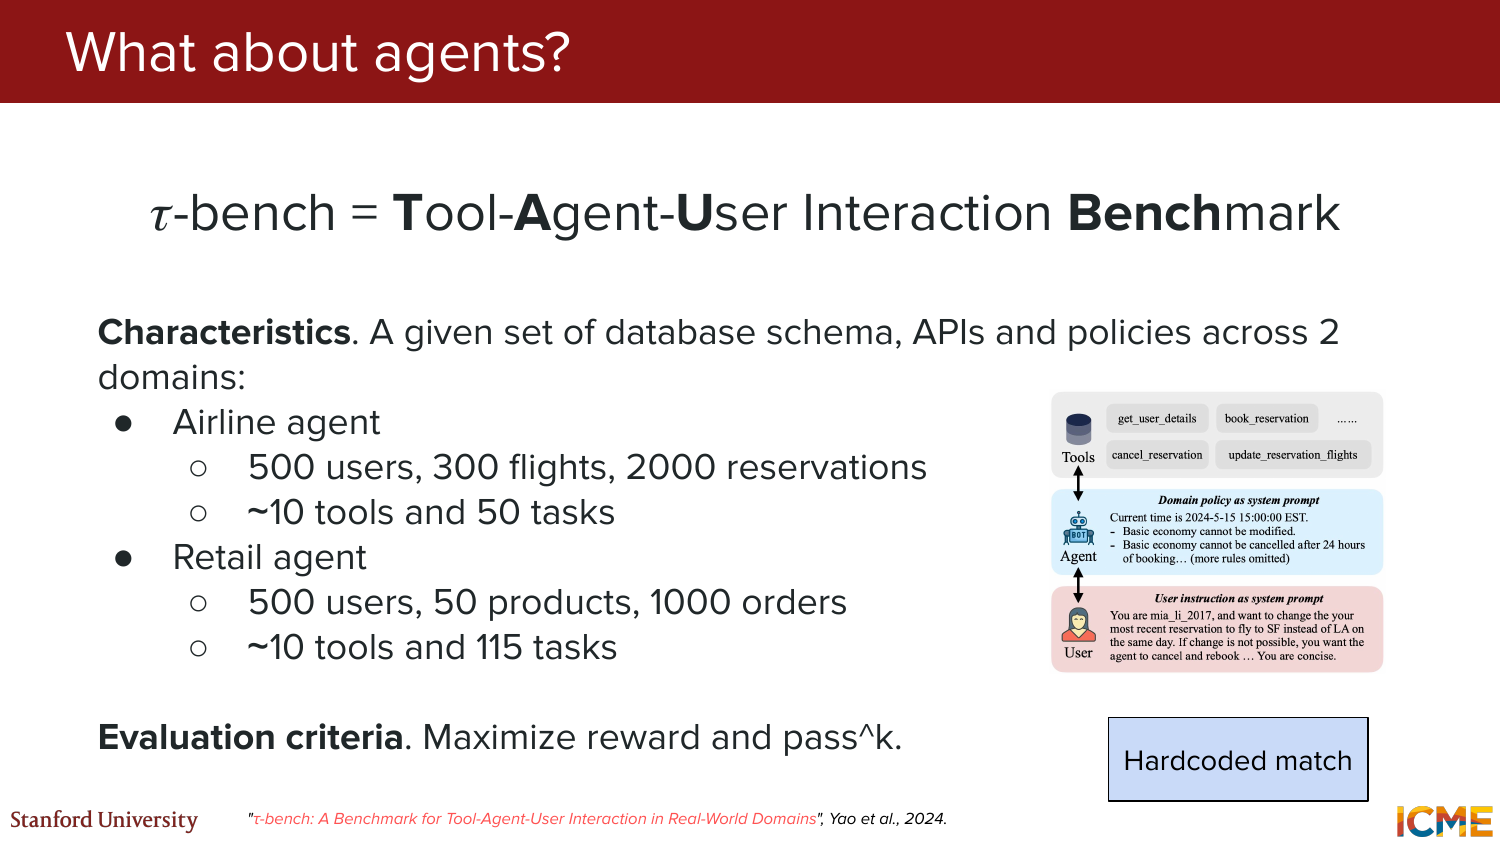
\includegraphics[width=0.92\textwidth]{pdf_pages/page-153.png}
\caption{$\tau$-bench 的课程示意图：在 airline / retail 两个领域中给 agent 提供工具、数据库状态与策略约束，评价是否稳定完成任务。}
\end{figure}

$\tau$-bench 是本讲最值得注意的新 benchmark，因为它把“工具 + 用户 + 环境状态”一起纳入。课程说明，这类 benchmark 往往要用语言模型模拟用户，因为对话会依赖前面步骤，无法像多项选择题那样静态写死。

评测 agent 时，讲者特别引入了一个可靠性视角：不是问“跑 $k$ 次至少成功一次的概率”，而是问“跑 $k$ 次是否次次都成功”。这对应课程里的 pass-hat-$k$ 直觉，可写成
\[
\mathrm{Pass}^{\wedge k} = \Pr(\text{all } k \text{ attempts succeed}).
\]

它体现的不是偶然可行性，而是可部署性。对 airline、retail 这类任务来说，偶尔成功远远不够，系统必须在重复执行中保持稳定。

\subsection{Pareto frontier、污染风险与 Goodhart 定律}

\begin{figure}[H]
\centering
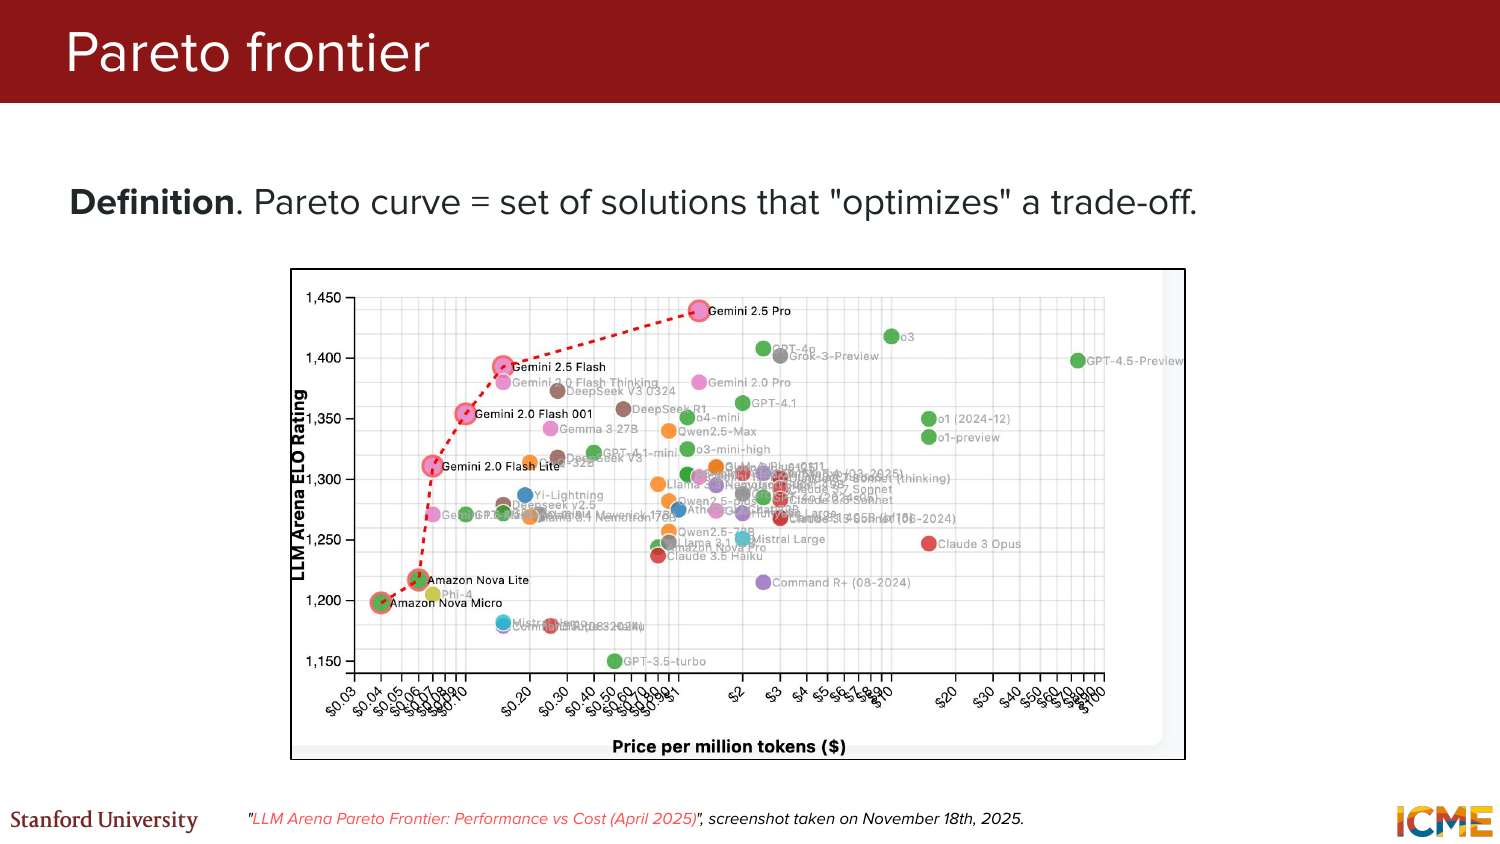
\includegraphics[width=0.92\textwidth]{pdf_pages/page-162.png}
\caption{课程中的 Pareto frontier 示意：把性能与成本放在同一张图上，寻找在既定预算下最优的模型选择。}
\end{figure}

课程后半段把 benchmark 从单个指标提升到系统选型视角。所谓 Pareto frontier，就是在给定两维目标下，任何一点如果要在一维继续提升，就必须在另一维付出代价。在 LLM 实践中，这通常意味着：更高质量往往更贵，而更便宜的模型常常需要牺牲部分能力。

但 benchmark 再多，也有两个必须警惕的陷阱。

第一是 \textbf{data contamination}。如果模型在训练时已经见过 benchmark 题面或答案，那么分数再高也不能真实反映泛化能力。因此课程提到的常见做法包括：为 benchmark 条目加 hash 标识、为 tool benchmark 维护 blocklist、以及在数学任务里尽量采用最新未公开试题。

第二是 \textbf{Goodhart's Law}：当一个度量本身成为优化目标，它就不再是好的度量。课程结尾用这句话提醒我们，benchmark 结果是有用的，但它只能近似用户价值，不能替代用户价值。

\begin{warningbox}{使用 benchmark 的正确姿势}
把 benchmark 看成 profile，而不是 verdict。它能帮助你理解模型在哪些维度上强、在哪些维度上弱，但不能替你决定“这个模型是否适合你的真实业务”。
\end{warningbox}

\subsection{本章小结}

Benchmark 的价值在于把模型能力投影到多个可比较轴上，包括知识、推理、代码、安全和 agent 可靠性。真正成熟的使用方式，是把 benchmark、成本、污染风险和真实用户目标一起考虑，而不是盯着单一排行榜。

\section{总结与延伸}

第 8 讲把“评测”从一个看似辅助性的环节，提升为 LLM 系统设计的中轴。没有评测，训练目标无法闭环；没有评测，RAG、tool calling、agents 的复杂系统也无法可靠迭代。

整讲可以压缩成三层逻辑：

\begin{enumerate}
\item 人工评分最接近真实价值，但昂贵、主观、慢；
\item Rule-based metrics 便宜可复现，但只覆盖任务的一部分；
\item LLM-as-a-Judge 扩展了自动化评测的语义能力，但自身也带有偏差，必须被人工校准。
\end{enumerate}

当我们把评测对象从单轮回答推进到 tool use 和 agent loop 时，课程进一步说明：好的指标不只是为了排名，更是为了诊断。它应该帮助我们定位错误发生在哪一层，理解系统在什么场景里会失败，以及这个失败到底会不会伤害真实用户。

如果把这一讲转成实践原则，可以记成五条：

\begin{enumerate}
\item 先定义你关心的维度，再选指标，不要反过来。
\item 人工评分要抽样保留，因为它是最终校准源。
\item Judge model 要被当作另一个会偏的模型，而不是神谕。
\item Agent 评测必须看可靠性，而不是偶尔成功率。
\item Benchmark 只给剖面，不给真理。
\end{enumerate}

顺着这个视角往下看，最后一讲就不再只是技术清单，而是要回答一个更大的问题：当我们把整个季度的内容拼起来，2025 年的大模型系统正在往哪里走，哪些趋势只是热点，哪些趋势真的可能改变体系结构与产品形态。

\end{document}
